\documentclass[english]{article}
\usepackage[utf8]{inputenc}
\usepackage[a4paper, left=3cm, right=3cm, top=4cm]{geometry}

% Language & links
\usepackage[english]{babel}
\usepackage[hidelinks]{hyperref}
\usepackage{etoolbox}

% Math
\usepackage{amsmath, amsfonts, amssymb, mathtools}
\usepackage{mathrsfs}      % script letters
\usepackage{physics}       % physics notation
\usepackage{tikz-cd}       % commutative diagrams
\usepackage{amsthm}        % proof

% Figures
\usepackage{graphicx} 
\usepackage{caption}
\usepackage{subcaption}
\usepackage[table,dvipsnames]{xcolor}
\usepackage{float}

% Tables
\usepackage{array}
\usepackage{multirow}
\usepackage{colortbl}
\usepackage{hhline}
\usepackage{booktabs}
\usepackage{booktabs}
\usepackage[table]{xcolor}
\usepackage{listings}
\usepackage{xcolor}  % Optional: for custom colors
% Layout
\usepackage{tcolorbox}     % colored boxes
\usepackage{enumitem}      % custom lists
\usepackage{epigraph}      % quotes at section start
\usepackage{setspace}

% Units
\usepackage[separate-uncertainty = true]{siunitx}

% Code
\usepackage{minted}

% Appendix
\usepackage[toc]{appendix}

% Bibliography
\usepackage{csquotes}
\usepackage[backend=biber,style=numeric]{biblatex} 
\addbibresource{references.bib}

% Fix physics + siunitxW
\AtBeginDocument{\RenewCommandCopy\qty\SI}
\ExplSyntaxOn
\msg_redirect_name:nnn {siunitx}{physics-pkg}{none}
\ExplSyntaxOff

\setlength{\parindent}{0pt} % No carriage return
\onehalfspacing     % Spaziatura

\makeatletter
\def\course#1{\gdef\@course{#1}}
\def\@course{} % default value

\def\supervisor#1{\gdef\@supervisor{#1}}
\def\@supervisor{} % default value

\def\@maketitle{%
    \newpage
    \null
    \begin{center}
        % Logo
        
\includegraphics[width=1\linewidth]{img/ictp-logo.jpg}\par\vspace{1cm}
        
        % Titolo
        {\huge\scshape \@title \par}\vspace{0.5cm}
        \rule{0.7\linewidth}{0.5pt}\vspace{1cm}
    \end{center}
    
    \begin{flushright}
        {\Large\bfseries \@author \par}
        {\sffamily \@course \par}
        \vspace{0.5cm}
        {\Large Supervisor: \@supervisor \par}
        \vspace{0.5cm}
        {\Large \@date \par}
    \end{flushright}
}
\makeatother

\title{Using Closed-loop Learning as an evaluator of clustering quality}
\author{Cerioli Gabriele}
\supervisor{Prof. Matteo Marsili}
\date{November 2025}

\begin{document}
\maketitle
\section{Measuring the fluctuations of the centroids}

We can take the KMeans algorithm as an example.
The closed-loop learning (CLL) algorithm is iterative, with the following steps in each cycle:
\begin{itemize}
    \item Apply KMeans clustering to the dataset, obtaining a hard labeling of the points.
    \item For each cluster, compute the mean and variance; this defines a mixture of Gaussians, one Gaussian per cluster.
    \item Generate $M$ synthetic points from the Gaussian mixture defined above and add these points to the dataset.
    \item Repeat the process, with the dataset growing at each step.
\end{itemize}

For example this is what happens to a KMeans clustering of the Iris Dataset after a CLL of 200 steps with $M=20$:

\begin{figure}[H]
  \centering
  \begin{minipage}{0.49\textwidth}
    \centering
    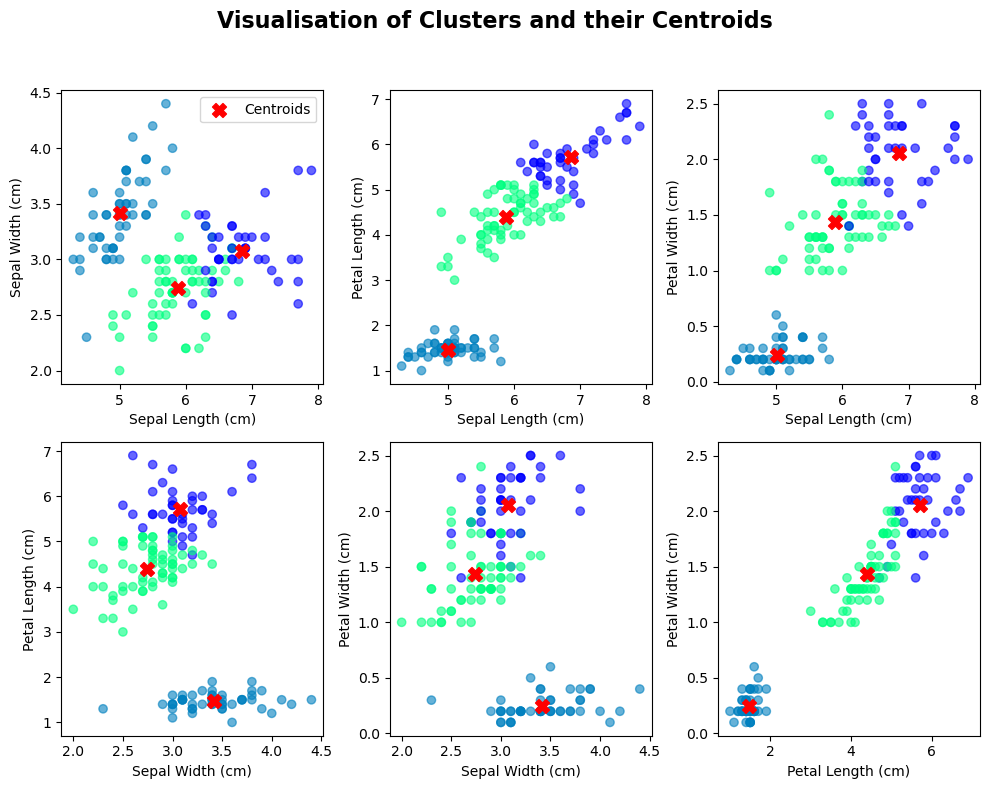
\includegraphics[width=\linewidth]{img/first_kmeans_clustering.png}
    \caption{Before CLL}
    \label{fig:iris_before}
  \end{minipage}\hfill
  \begin{minipage}{0.49\textwidth}
    \centering
    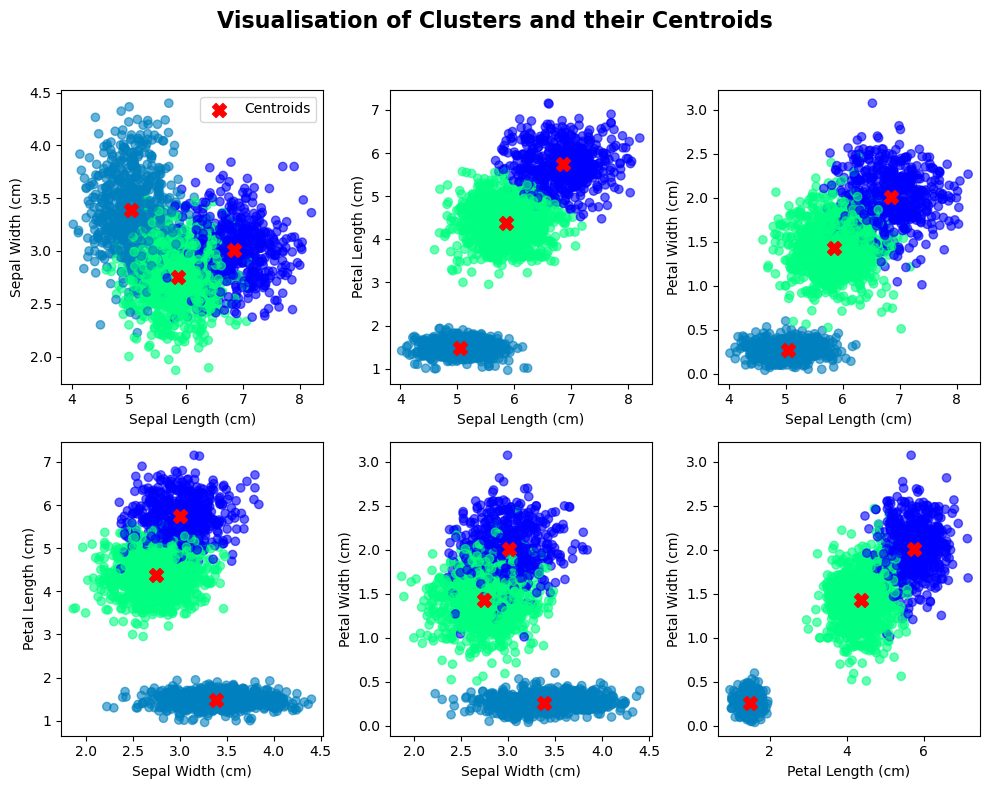
\includegraphics[width=\linewidth]{img/final_clustering.png}
    \caption{After CLL (200 steps, $M=20$)}
    \label{fig:iris_after}
  \end{minipage}
\end{figure}

We expect that, after the CLL algorithm has converged, the cluster centers will have shifted slightly. \\

Assuming that CLL is a valid, convergent clustering procedure, we can assess the quality of the original method (here KMeans) by measuring the displacements and fluctuations of the centroids.

We can plot the norm of the displacements of the centroids from initial conditions at each step of the algorithm:

\begin{figure} [H]
\centering
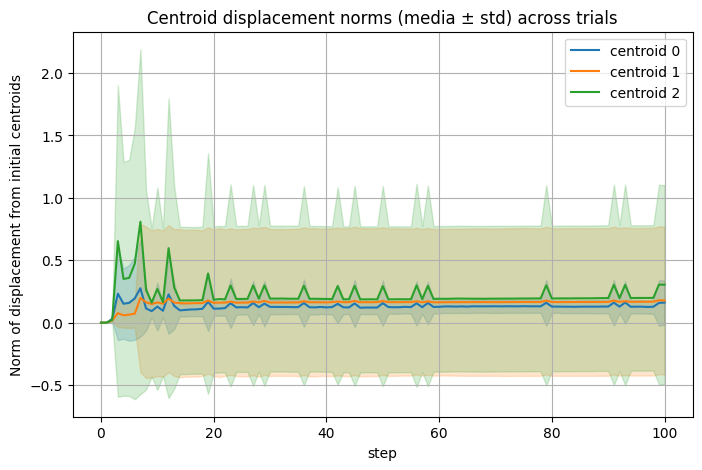
\includegraphics[width=\linewidth]{img/displacement of centroids.png}
\end{figure}



\section{Comparison with distance between clusters}
The idea is that if we compare the displacements of the cluster $\delta$ after the CLL exection and the original distances $D$ between the clusters we can evaluate the quality of the clusterisation.\\

We expect that:
\begin{itemize}
    \item the smaller the ratio $\frac{\delta}{D}$ the better the clusterisation
    \item If the displacements $\delta$ are comparable with the original distances $D$, we consider it a poor clusterisation.
\end{itemize}
Given $N$ clusters we can define the cluster quality $Q$ as:
\begin{equation*}
Q= \frac{\sum_{i=1}^{N}\frac{\delta_i}{D_i}}{N}
\end{equation*}
where $D_i$ is the mean of the distances between cluster $i$ and all the others, this is to say $D_i=\sum_{j=1}^{N}\frac{ \left\| \overrightarrow{x_i}-\overrightarrow{x_j} \right\| }{N-1}$ where $\overrightarrow{x_i}$ is the centroid of cluster $i$\\

For example in the case of a KMeans clusterisation of the Iris Dataset we get:
\begin{equation*}
    Q=\frac{\frac{0.083}{3.39}+\frac{0.057}{4.17}+\frac{0.030}{2.57}}{3}=0.017
\end{equation*}


While in the case of a Gaussian Mixtures clustering of the Iris dataset we get:

\begin{figure}[H]
  \centering
  \begin{minipage}{0.49\textwidth}
    \centering
    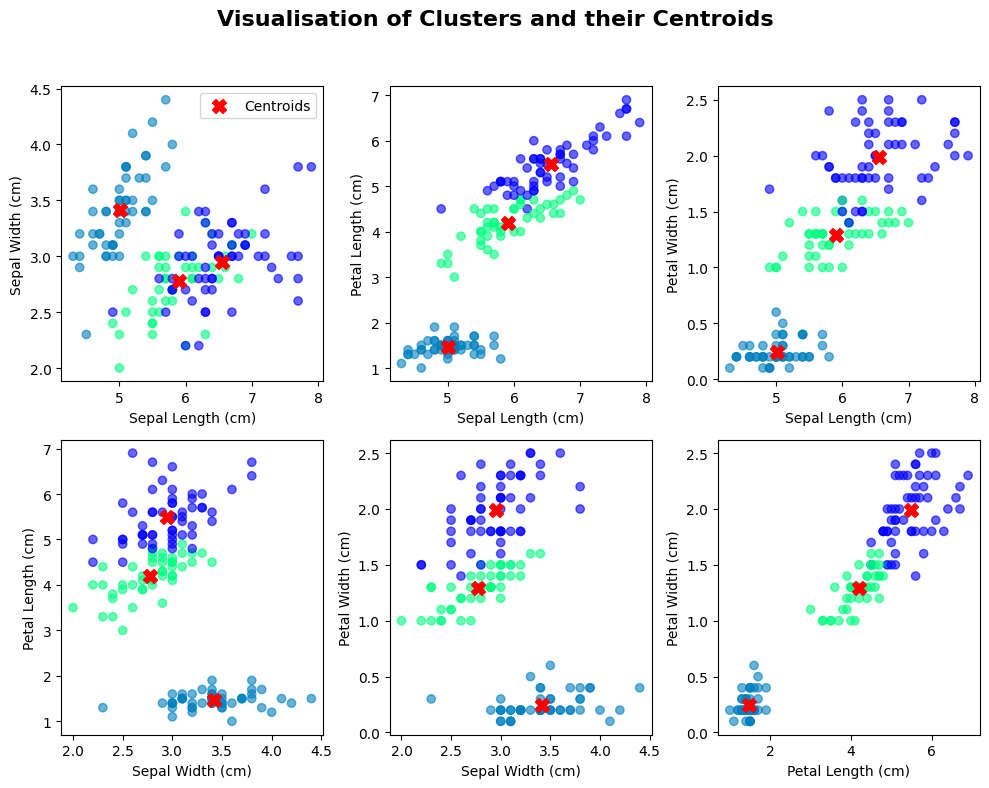
\includegraphics[width=\linewidth]{img/GM_iris.png}
    \caption{Gaussian Mixtures before CLL}
    \label{fig:iris_before}
  \end{minipage}\hfill
  \begin{minipage}{0.49\textwidth}
    \centering
    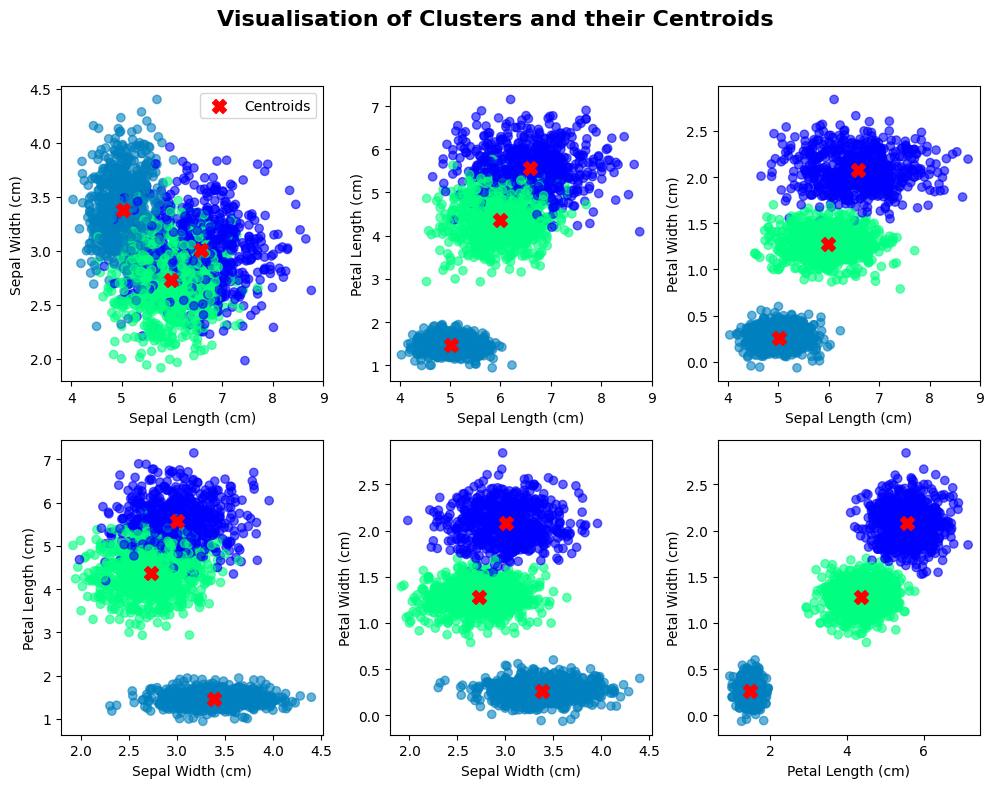
\includegraphics[width=\linewidth]{img/GM+CLL_iris.png}
    \caption{Gaussian Mistures after CLL (200 steps, $M=20$)}
    \label{fig:iris_after}
  \end{minipage}
\end{figure}

We get these displacements of the centroids at each step:

\begin{figure} [H]
    \centering
    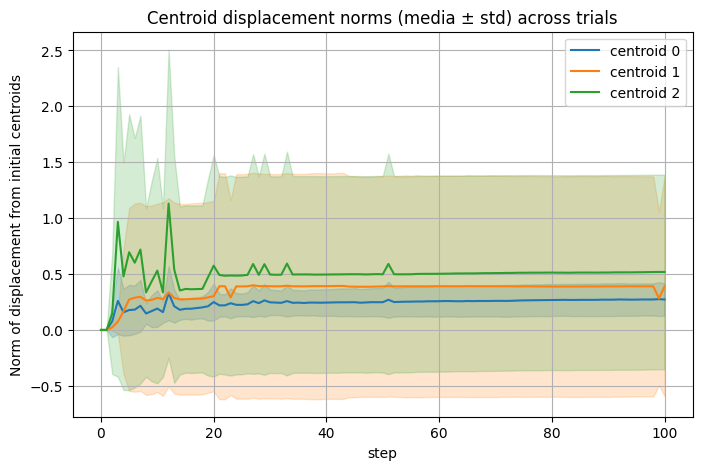
\includegraphics[width=\linewidth]{img/GM_displacement.png}
    \caption{Displacements of centroids with Gaussian Mixtures on Iris database}
\end{figure}
and we get a quality of:
\begin{equation*}
    Q=\frac{\frac{0.131}{3.15}+\frac{0.044}{3.19}+\frac{0.202}{2.38}}{3}=0.046
\end{equation*}
much worse than the quality of the KMeans clustering of Iris Database.

\section{Using Q to find the optimal number of clusters}
Can we use the value of Q to find the optimal number of clusters in a dataset. \\

We can try to iterate the Q estimation with different numbers of clusters, in the simple case of the Iris Dataset we get:

\begin{figure} [H]
\centering
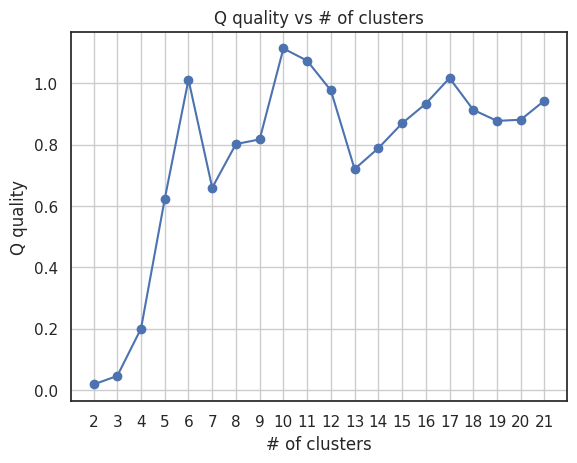
\includegraphics[width=\linewidth]{img/number_clusters.png}
\end{figure}
In this case the CLL seems useful to estimate the optimal number of clusters.
\end{document}